%%%
% Plantilla de Memoria
% Modificación de una plantilla de Latex de Nicolas Diaz para adaptarla 
% al castellano y a las necesidades de escribir informática y matemáticas.
%
% Editada por: Mario Román
%
% License:
% CC BY-NC-SA 3.0 (http://creativecommons.org/licenses/by-nc-sa/3.0/)
%%%

%%%%%%%%%%%%%%%%%%%%%%%%%%%%%%%%%%%%%%%%%
% Thin Sectioned Essay
% LaTeX Template
% Version 1.0 (3/8/13)
%
% This template has been downloaded from:
% http://www.LaTeXTemplates.com
%
% Original Author:
% Nicolas Diaz (nsdiaz@uc.cl) with extensive modifications by:
% Vel (vel@latextemplates.com)
%
% License:
% CC BY-NC-SA 3.0 (http://creativecommons.org/licenses/by-nc-sa/3.0/)
%
%%%%%%%%%%%%%%%%%%%%%%%%%%%%%%%%%%%%%%%%%

%----------------------------------------------------------------------------------------
%	PAQUETES Y CONFIGURACIÓN DEL DOCUMENTO
%----------------------------------------------------------------------------------------
%%% Configuración del papel.
% microtype: Tipografía.
% mathpazo: Usa la fuente Palatino.
\documentclass[a4paper, 11pt]{article}
\usepackage[protrusion=true,expansion=true]{microtype}
\usepackage{mathpazo}


% Indentación de párrafos para Palatino
\setlength{\parindent}{0pt}
  \parskip=8pt
\linespread{1.05} % Change line spacing here, Palatino benefits from a slight increase by default


%%% Castellano.
% noquoting: Permite uso de comillas no españolas.
% lcroman: Permite la enumeración con numerales romanos en minúscula.
% fontenc: Usa la fuente completa para que pueda copiarse correctamente del pdf.
\usepackage[spanish,es-noquoting,es-lcroman]{babel}
\usepackage[utf8]{inputenc}
\usepackage[T1]{fontenc}
\selectlanguage{spanish}


%%% Gráficos
\usepackage{graphicx} % Required for including pictures
\usepackage{wrapfig} % Allows in-line images
\usepackage[usenames,dvipsnames]{color} % Coloring code

%%%%%%% LICENCIA

\usepackage[scale=2]{ccicons}

%%% Matemáticas
\usepackage{amsmath}


%%% Bibliografía
\makeatletter
\renewcommand\@biblabel[1]{\textbf{#1.}} % Change the square brackets for each bibliography item from '[1]' to '1.'
\renewcommand{\@listI}{\itemsep=0pt} % Reduce the space between items in the itemize and enumerate environments and the bibliography
\usepackage{hyperref}
\hypersetup{
	colorlinks   = true,    % Colours links instead of ugly boxes
	urlcolor     = red,    % Colour for external hyperlinks
	linkcolor    = red,    % Colour of internal links
	citecolor    = blue      % Colour of citations
}

%%% CÓDIGO

\usepackage{listings}   
\usepackage{xcolor}
\lstdefinestyle{customc}{	
	backgroundcolor=\color{white},    % choose the background color; you must add \usepackage{color} or \usepackage{xcolor}; should come as last argument
	basicstyle=\footnotesize\ttfamily,% the size of the fonts that are used for the code
	breakatwhitespace=false,          % sets if automatic breaks should only happen at whitespace
	breaklines=true,                  % sets automatic line breaking
	captionpos=b,                     % sets the caption-position to bottom
    commentstyle=\itshape\color{purple!40!black},     % comment style
	deletekeywords={...},             % if you want to delete keywords from the given language
	escapeinside={\%*}{*)},           % if you want to add LaTeX within your code
	extendedchars=true,               % lets you use non-ASCII characters; for 8-bits encodings only, does not work with UTF-8
	frame=single,	                  % adds a frame around the code
	keepspaces=true,                  % keeps spaces in text, useful for keeping indentation of code (possibly needs columns=flexible)
	keywordstyle=\bfseries\color{green!40!black},       % keyword style
	language=C,                       % the language of the code
	morekeywords={*,...},             % if you want to add more keywords to the set
	numbers=left,                     % where to put the line-numbers; possible values are (none, left, right)
	numbersep=5pt,                    % how far the line-numbers are from the code
	numberstyle=\tiny\color{gray},    % the style that is used for the line-numbers
	rulecolor=\color{black},          % if not set, the frame-color may be changed on line-breaks within not-black text (e.g. comments (green here))
	showspaces=false,                 % show spaces everywhere adding particular underscores; it overrides 'showstringspaces'
	showstringspaces=false,           % underline spaces within strings only
	showtabs=false,                   % show tabs within strings adding particular underscores
	stepnumber=2,                     % the step between two line-numbers. If it's 1, each line will be numbered
    stringstyle=\color{orange},       % string literal style
	tabsize=2,	                      % sets default tabsize to 2 spaces
	title=\lstname,                   % show the filename of files included with \lstinputlisting; also try caption instead of title
	identifierstyle=\color{blue}
}

\lstdefinestyle{customasm}{
	belowcaptionskip=1\baselineskip,
	frame=L,
	xleftmargin=\parindent,
	language=[x86masm]Assembler,
	basicstyle=\footnotesize\ttfamily,
	commentstyle=\itshape\color{purple!40!black},
}

\DeclareFixedFont{\ttb}{T1}{txtt}{bx}{n}{8} % for bold
\DeclareFixedFont{\ttm}{T1}{txtt}{m}{n}{8}  % for normal


\lstdefinestyle{customPY}{
	language=Python,
	basicstyle=\ttm,
	otherkeywords={self},             % Add keywords here
	keywordstyle=\ttb\color{blue},
	emph={MyClass,__init__},          % Custom highlighting
	emphstyle=\ttb\color{red},    % Custom highlighting style
	stringstyle=\color{orange},
	frame=tb,                         % Any extra options here
	showstringspaces=false       
}

\lstset{escapechar=@,style=customc}




%----------------------------------------------------------------------------------------
%	TÍTULO
%----------------------------------------------------------------------------------------
% Configuraciones para el título.
% El título no debe editarse aquí.
\renewcommand{\maketitle}{
  \begin{flushright} % Right align
  
  {\LARGE\@title} % Increase the font size of the title
  
  \vspace{50pt} % Some vertical space between the title and author name
  
  {\large\@author} % Author name
  \\\@date % Date
  \vspace{40pt} % Some vertical space between the author block and abstract
  \end{flushright}
}

%% Título
\title{\textbf{Práctica 3}\\ % Title
Estructura de computadores} % Subtitle

\author{\textsc{Francisco Navarro Morales} % Author
\\{\textit{Universidad de Granada}}} % Institution

\date{\today} % Date





%----------------------------------------------------------------------------------------
%	DOCUMENTO
%----------------------------------------------------------------------------------------

\begin{document}
	


\maketitle % Print the title section

%% Resumen (Descomentar para usarlo)
\renewcommand{\abstractname}{Resumen} % Uncomment to change the name of the abstract to something else
%\begin{abstract}
% Resumen aquí
%\end{abstract}

%% Palabras clave
%\hspace*{3,6mm}\textit{Keywords:} lorem , ipsum , dolor , sit amet , lectus % Keywords
%\vspace{30pt} % Some vertical space between the abstract and first section


%% Índice
{\parskip=2pt
  \tableofcontents
}
\ccLogo
\ccAttribution
\ccShareAlike
\ccNonCommercialEU	


%%% Inicio del documento

\section{PopCount.}
El objetivo de esta primera parte es comparar distintas implementaciones de un algoritmo PopCount (cuyo objetivo es calcular el peso Hamming\footnote{Número de unos que tiene el número en binario.} de una lista de números) para comprobar hasta qué punto puede o no ser útil escribir ciertos programas (o partes de un programa) en ensamblador.
\subsection{Primera y segunda versión.}
Basándome en las transparencias vistas en clase (tr.43 y 38) realizo una primera versión (Figura~\ref{primera versión}) con un bucle for y una segunda (Figura \ref{segunda versión}) con un bucle while para ir extrayendo y acumulando bits. Los resultados obtenidos (Figura~\ref{1y2}) indican una diferencia (favorable para la segunda versión) de unos 0.03 segundos. 
\begin{figure}[!hbp]
	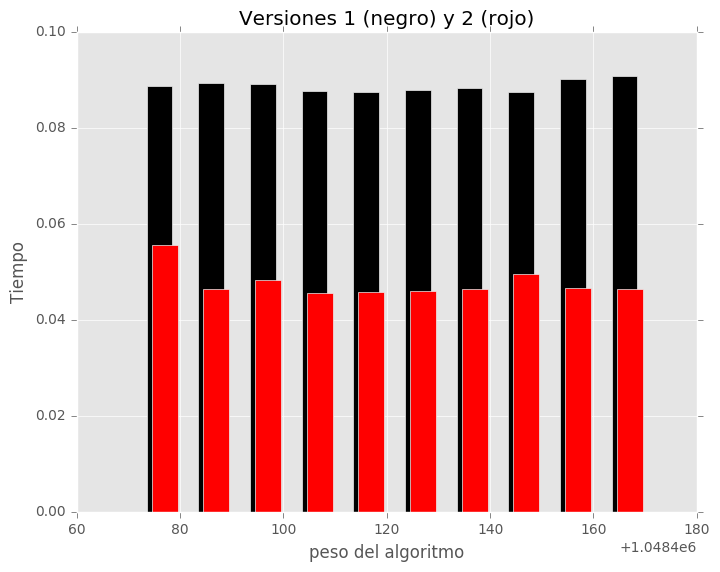
\includegraphics[scale=0.6]{1y2.png}
	\caption{1 y 2	\label{1y2}}
\end{figure}
La principal diferencia entre estas dos implementaciones es que la primera utiliza un iterador para el bucle for, que debe ser incrementado en cada iteración del bucle y que se utiliza para comprobar si se ha terminado de procesar el número ; mientras que la segunda versión prescinde de dicho iterador y se limita a comprobar en cada iteración si el número es mayor que cero (ya que en cada iteración los bits del número son desplazados a la derecha y, por tanto, el número disminuye hasta ser cero). Es decir, que a pesar de que la diferencia es mínima (simplemente el incremento de una variable en cada iteración del bucle), ya se produce un cambio notable en los tiempos de ejecución de estas versiones.

\subsection{Tercera versión.}
La siguiente versión a comparar consiste en introducir un tramo (dentro del programa escrito en C) de instrucciones en ensamblador, con el objetivo de ver si realmente merece la pena introducir este tipo de instrucciones en nuestros programas. Dado que el bit desplazado acaba en el acarreo (debido a la forma en que actúa la orden SHR), lo podemos sumar de ahí mismo y nos ahorramos algunas instrucciones. Dado que ya hemos comprobado que la segunda versión es más rápida que la primera, es interesante comparar esta tercera versión (Figura~\ref{tercera versión}) solo con la segunda. (Figura~\ref{2y3})
\begin{figure}[!hbp]
	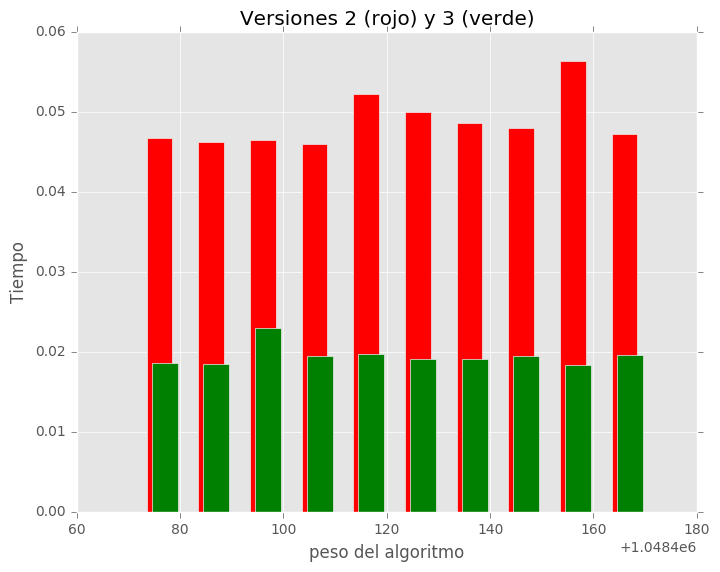
\includegraphics[scale=0.6]{2y3.png}
	\caption{ 2 y 3 	\label{2y3}}
\end{figure}
\begin{figure}[!hbp]
	\lstinputlisting[language=c]{primerafor.c}
	\caption{Código de la primera versión 	\label{primera versión}}
\end{figure}

\begin{figure}[!hbp]
	\lstinputlisting[language=c]{segundawhile.c}

	\caption{Código de la segunda versión 	\label{segunda versión}}
\end{figure}

\begin{figure}[!hbp]
	\lstinputlisting[language=c]{terceraADC.c}
	\caption{Código de la tercera versión 	\label{tercera versión}}
\end{figure}



\subsection{Cuarta versión.}
La cuarta versión (Figura~\ref{cuarta versión}), consiste en aplicar la máscara 0x01010... a cada número de forma que se vayan acumulando los bits de cada byte en una nueva variable y sumar en árbol (de esta forma se cuenta un bit por byte en cada iteración y el número de iteraciones disminuye). Esta cuarta versión debería ser más rápida que las anteriores (Figura \ref{3y4}) y nos demostraría, de ser así, lo difícil que es superar a GCC en cuanto a optimización. 

\begin{figure}[!hbp]
	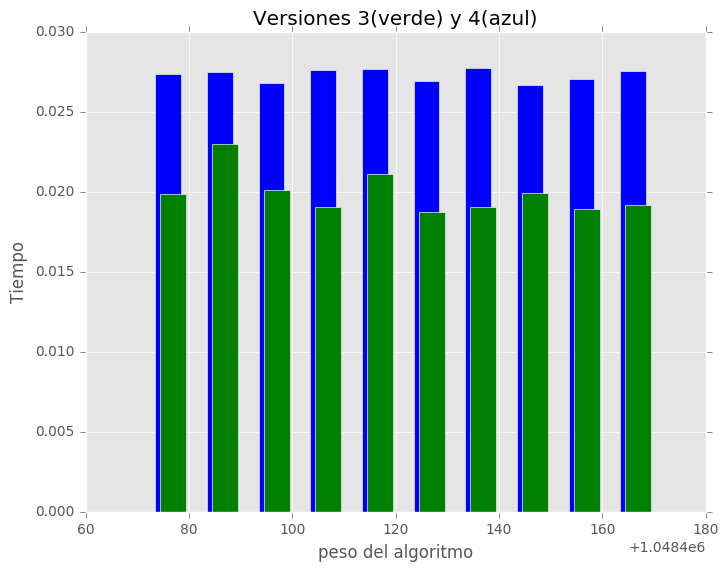
\includegraphics[scale=0.6]{3y4.png}
	\caption{1 y 2	\label{3y4}}
\end{figure}

Al contrario de lo que cabría esperar, la versión escrita en C con algunos arreglos en ASM es algo mejor que el programa (mejor pensado en ASM) escrito totalmente en esamblador. 

\begin{figure}[!hbp]
	\lstinputlisting[language=c]{cuartamask.c}
	\caption{Código de la cuarta versión \label{cuarta versión}}
\end{figure}


\subsection{Optimizaciones.}
\begin{figure}[!hbp]
	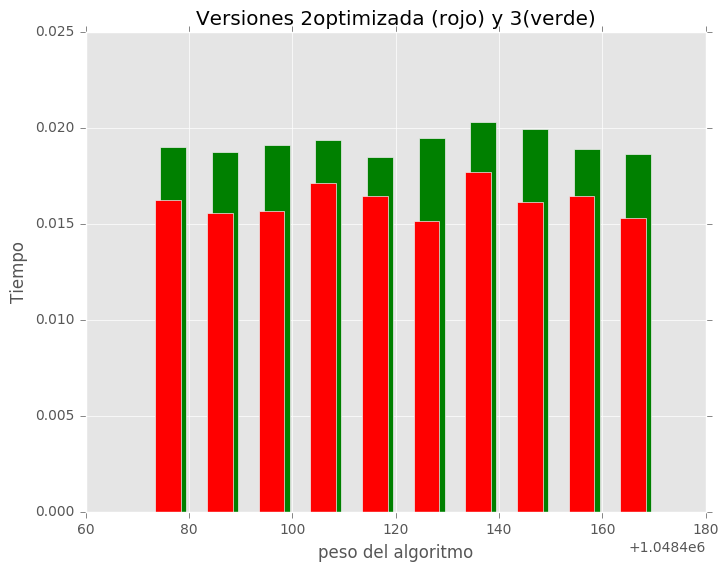
\includegraphics[scale=0.6]{2y3op.png}
	\caption{2 y 3 optimizada	\label{2y3op}}
	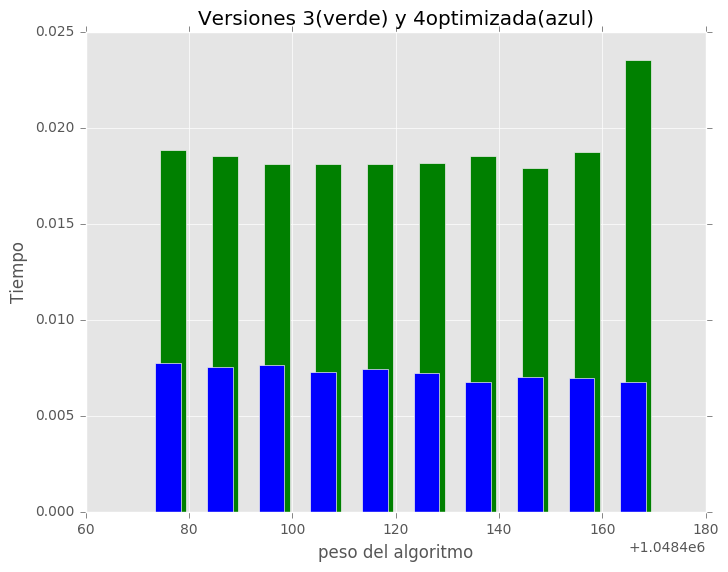
\includegraphics[scale=0.6]{3y4op.png}
	\caption{3 y 4optimizada	\label{3y4op}}
\end{figure}

Antes de avanzar más, es interesante plantearse el modo de compilación de los programas escritos en C; ya que si compilamos estos aumentando las optimizaciones que genera GCC podremos obtener tiempos mucho mejores. Algunos ejemplos:
En la (Figura \ref{2y3op}), se puede apreciar que la versión 2 (solo código en C) ya supera a la 3, solo aplicando las optimizaciones (-O3). Así mismo, la Figura \ref{3y4op} nos muestra que, pidiendo a GCC que optimice las versiones 3 y 4 (para optimizar la versión 3 hay que cambiar la etiqueta << init3 >> por << 0  >> o nos dará un error de compilación") 




\subsection{Quinta versión.}
La última versión a comparar la podemos encontrar en Github, en la dirección: 
\href{https://github.com/WojciechMula/sse-popcount/blob/master/original/ssse3_popcount.c}{PopCount-SSSE}
Y una explicación gráfica en : \href{https://swad.ugr.es/swad/tmp/8bjaqPAeqvL0feJfeyxpCOQWZuXTEo-5cDNq33cXc7s/popcount5.txt}{explicación del algoritmo}
Grosso modo, podríamos decir que se trata de una versión mucho más compleja (y premeditada) que la de la versión 4, que realiza sumas de bites en paralelo y utiliza los deplazamientos para agilizar el proceso. Si lo comparamos con la versión optimizada de la cuarta implementación (La mejor hasta ahora) el resultado es el que se muestra en la figura \ref{4y5}. 
\begin{figure}[!htbp]
	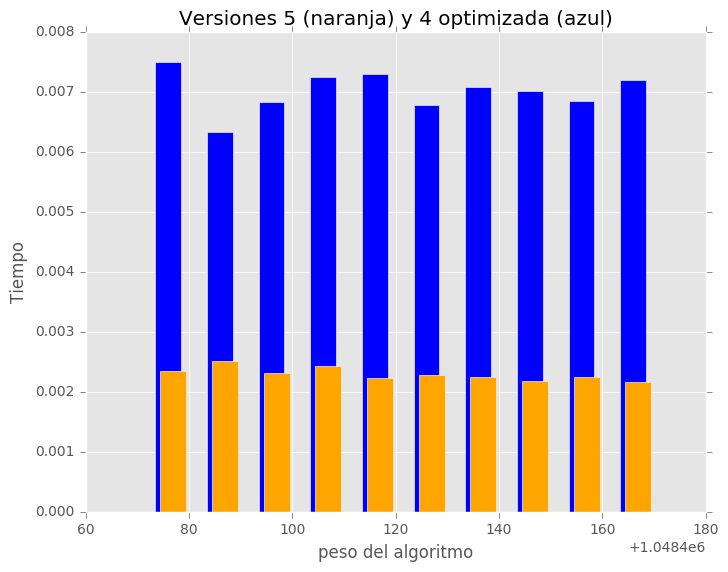
\includegraphics[scale=0.6]{4y5.png}
	\caption{4 y 5	\label{4y5}}
\end{figure}
\pagebreak
\section{Parity}
En esta segunda práctica realizaremos un procedimiento similar al anterior, pero esta vez con un algoritmo que calcula la cantidad de números con paridad impar del vector. 

\subsection{Primera y segunda versión}
Las dos primeras versiones son algo similares a las del algoritmo PopCount, con un bucle for y un bucle while respectivamente.
\begin{figure}[!hbp]
	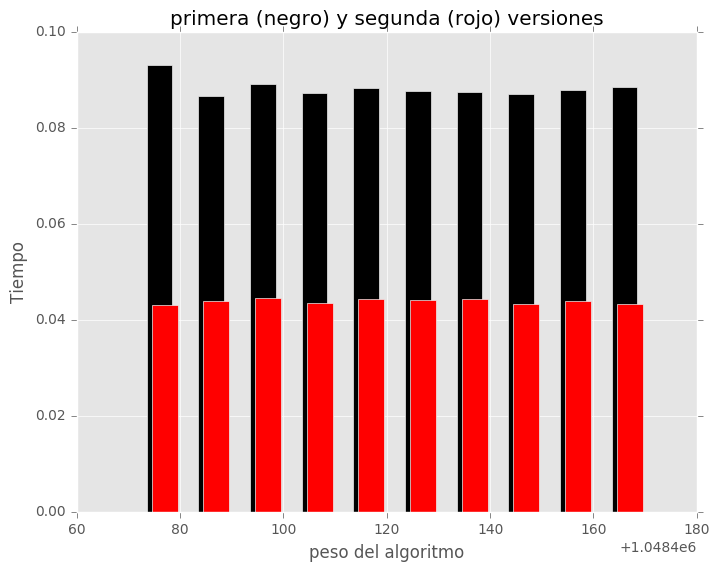
\includegraphics[scale=0.6]{1y2p.png}
	\caption{1 y 2	\label{1y2p}}
\end{figure} 

Se puede apreciar fácilmente una cierta mejoría al usar el bucle while por las mismas razones que en el caso del PopCount.

No es demasiado interesante comparar los distintos niveles de optimización puesto que, -O1 y -O2 dan resultados muy similares; bastante mejores, eso sí, que -O0.

\begin{figure}[!hbp]
	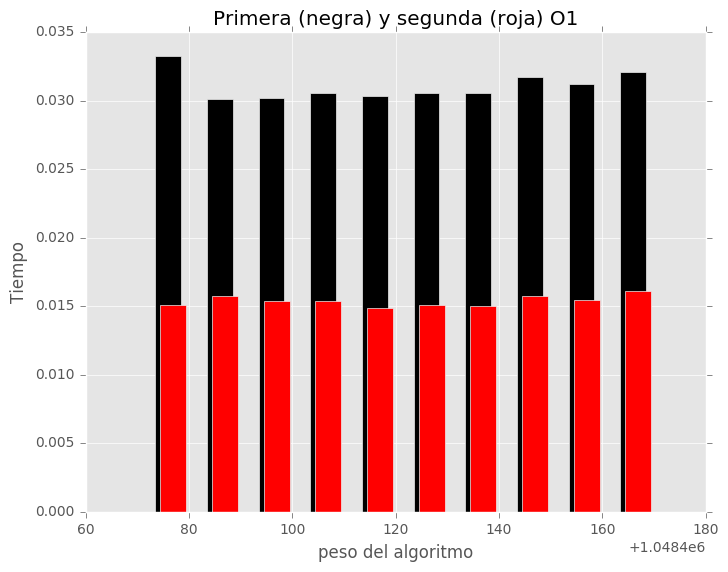
\includegraphics[scale=0.6]{1y2p_1.png}
	\caption{1 y 2	\label{1y2p_1}}
	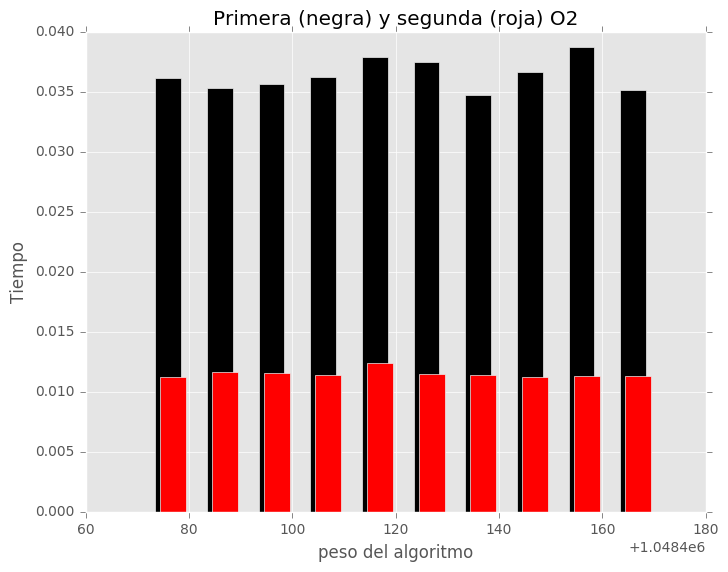
\includegraphics[scale=0.6]{1y2p_2.png}
	\caption{1 y 2	\label{1y2p_2}}
\end{figure}

\begin{figure}[!hbp]
	\lstinputlisting[language=c]{pprimera.c}
	\caption{Código de la primera versión 	\label{pprimera versión}}
\end{figure}

\begin{figure}[!hbp]
	\lstinputlisting[language=c]{psegunda.c}
	\caption{Código de la segunda versión 	\label{psegunda versión}}
\end{figure}

\subsection{Tercera versión}
Dado que lo que estamos contando es la cantidad de números con paridad impar podemos ahorrarlos la máscara para separar el bit menos significativo (que hacíamos en el bucle while en la versión 2) y limitarnos a aplicar dicha máscara al final del bucle, a la hora de sumar el resultado (cero o uno) al acumulador resultado. Es decir, lo que vamos haciendo es hacer la operación xor del número completo en cada iteración del bucle while (sin la máscara) pero en realidad lo que nos va a valer es sólo el bit menos significativo; los demás bits no nos interesan pero no importa, porque se van a perder trás el bucle while, al acumular los resultados. Aún sabiendo esto, las diferencias de tiempo entre la segunda y la tercera versión son mínimas, en los distintos grados de optimización quizá sea -O2 cuando más diferencia puedo apreciar.

\begin{figure}[!hbp]
	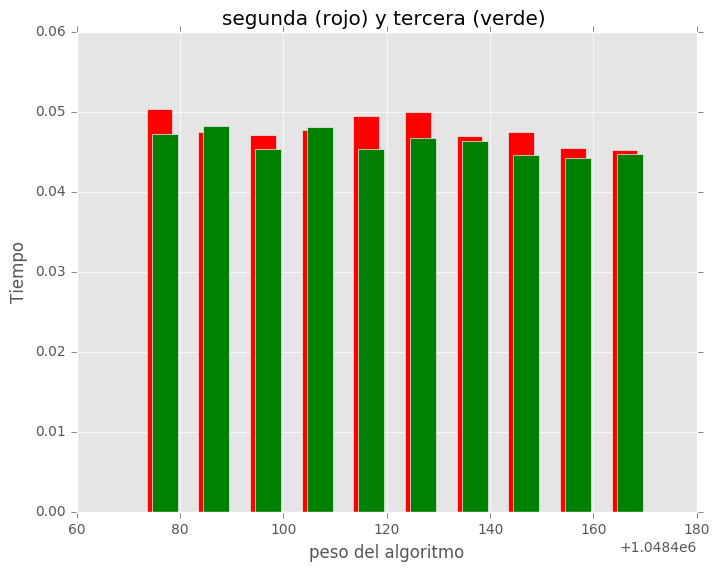
\includegraphics[scale=0.6]{2y3p.png}
	\caption{1 y 2	\label{2y3p}}
\end{figure} 
\begin{figure}[!hbp]
	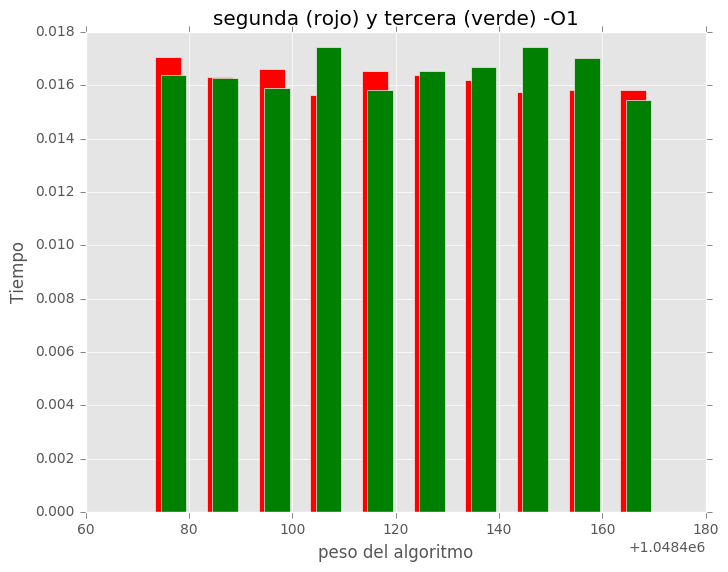
\includegraphics[scale=0.6]{2y3_1p.png}
	\caption{1 y 2	\label{2y3_1p}}
\end{figure} 
\begin{figure}[!hbp]
	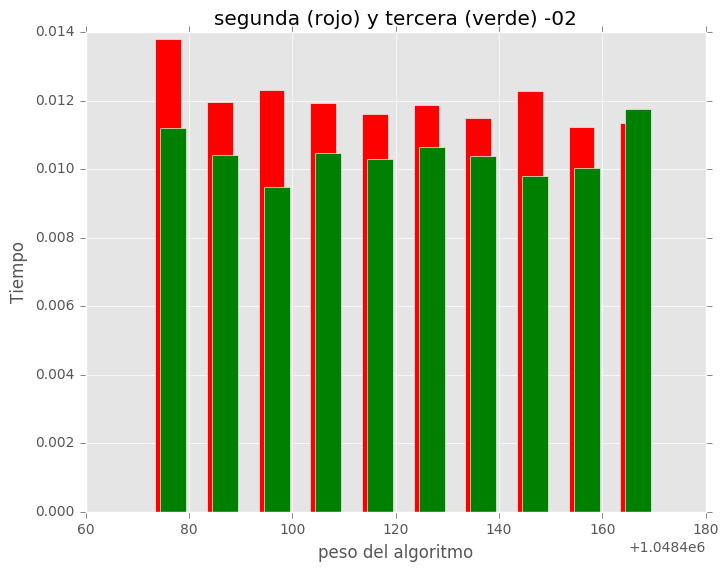
\includegraphics[scale=0.6]{2y3_2p.png}
	\caption{1 y 2	\label{2y3p_2}}
\end{figure} 
\begin{figure}[!hbp]
	\lstinputlisting[language=c]{ptercera.c}
	\caption{Código de la tercera versión (parity) 	\label{parity tercera versión}}
\end{figure}

\pagebreak
\subsection{Cuarta versión}
Esta vez, al igual que hicimos en el PopCount, vamos a intentar mejorar la implementación añadiendo un bloque ASM que hará uso de la orden SHR al igual que hicimos en el bloque ASM del algoritmo PopCount. Es interesante ver que, al compilar, el código obtenido en O1 es prácticamente el mismo que el de la versión anterior; sin embargo, sin optimización y con -O2 esta versión supera a la tercera.

\begin{figure}[!hbp]
	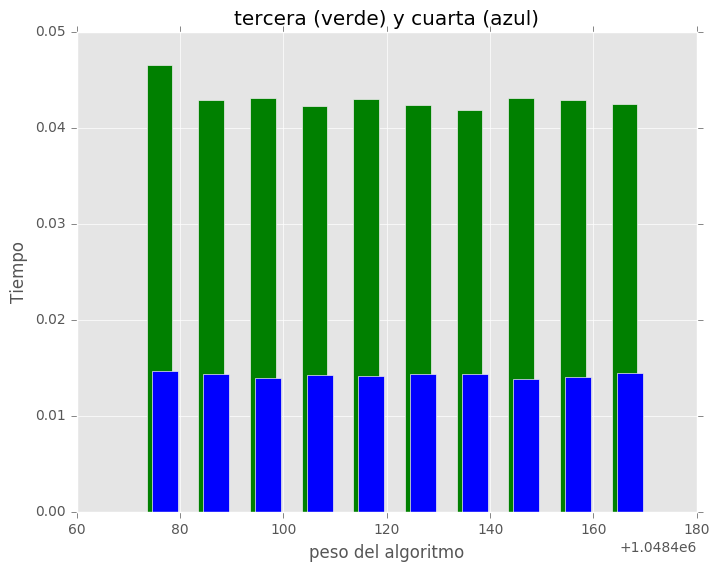
\includegraphics[scale=0.6]{3y4p.png}
	\caption{1 y 2	\label{3y4p}}
\end{figure} 
\begin{figure}[!hbp]
	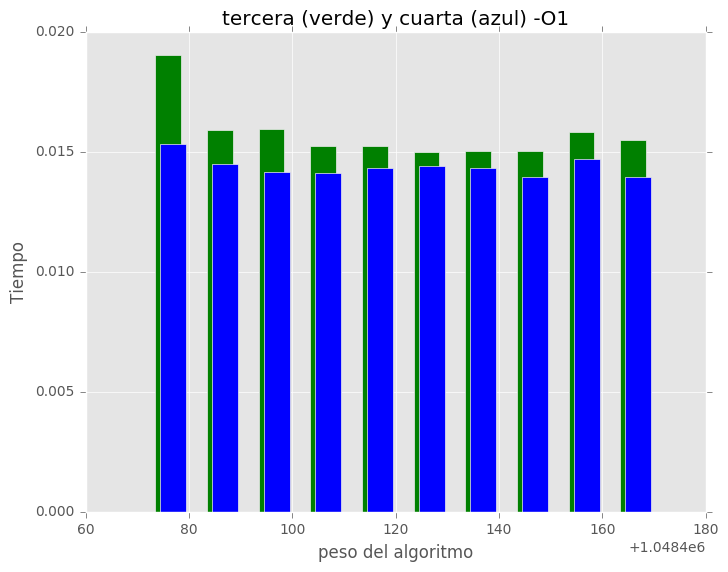
\includegraphics[scale=0.6]{3y4p_1.png}
	\caption{1 y 2	\label{3y4p_1p}}
\end{figure} 
\begin{figure}[!hbp]
	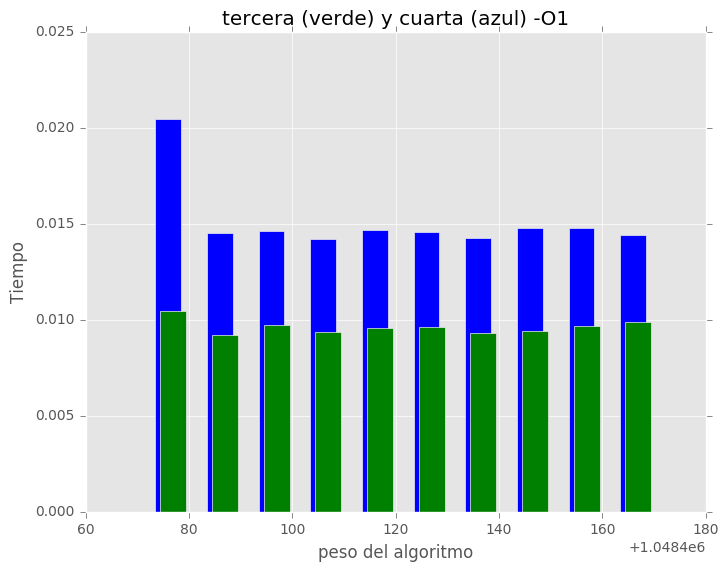
\includegraphics[scale=0.6]{3y4p_2.png}
	\caption{1 y 2	\label{3y4p_2}}
\end{figure}
\begin{figure}[!hbp]
	\lstinputlisting[language=c]{pcuarta.c}
	\caption{Código de la cuarta versión (parity)	\label{parity cuarta versión}}
\end{figure}
\pagebreak
\subsection{Quinta versión}
Al igual que hicimos con el algoritmo PopCount, podemos realizar una versión que realice la comprobación de paridad en árbol; es decir: dado que nuestro objetivo es saber si el número de dígitos uno es impar, podemos ir haciendo la operación xor del número consigo mismo (desplazándolo un poco cada vez) de forma que este se vaya partiendo en dos mitades las cuales se van sumando (suma exclusiva xor). Dado que la suma exclusiva devuelve un 1 si los dígitos sumados eran distintos y un 0 si eran iguales, cada vez que se sumen dos unos, estos se anularán (se volverán un cero), lo cual nos interesa puesto que queremos saber si hay un número impar de unos, pero no cuantos. Así, dado que cada vez el número se divide en partes más que pequeñas que se van sumando (xor), nos encontraremos en que al final tenemos en el bit menos significativo 1 o 0 dependiendo de si el número de unos iniciales era impar o no. El resto de los dígitos no tienen importancia. 
Aunque pudiera parecer que el algoritmo es mucho mejor que la versión anterior, si no planificamos bien como implementarlo y copilamos con O0, los resultados son incluso peores que los de la cuarta versión. No obstante, basta compilar con -O1 u -O2 para ver la mejoría.


\begin{figure}[!hbp]
	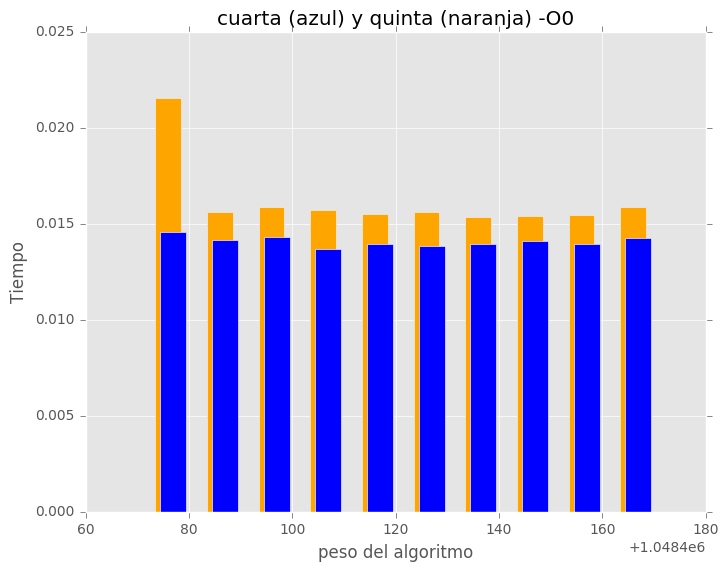
\includegraphics[scale=0.6]{4y5p.png}
	\caption{4 y 5	\label{4y5p}}
\end{figure} 
\begin{figure}[!hbp]
	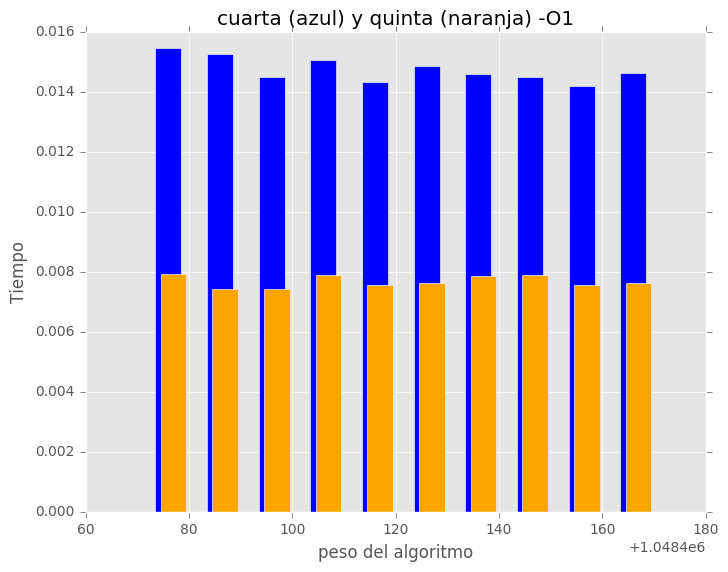
\includegraphics[scale=0.6]{4y5p_1.png}
	\caption{4 y 5	\label{4y5p_1}}
\end{figure} 
\begin{figure}[!hbp]
	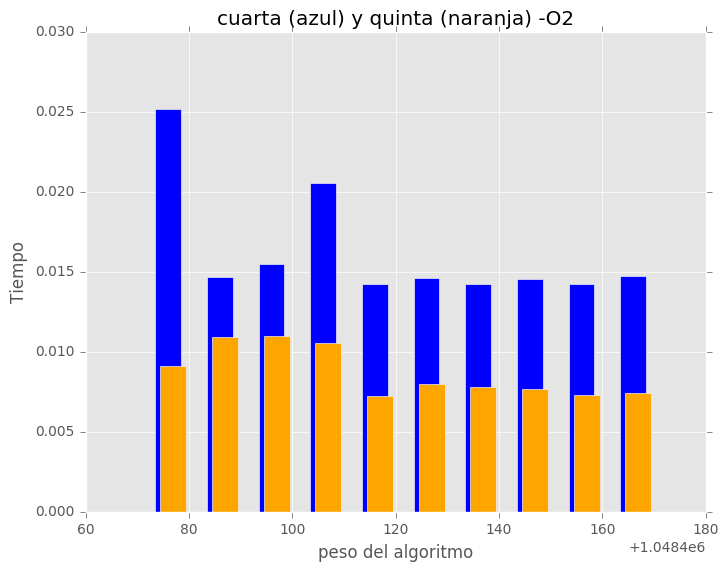
\includegraphics[scale=0.6]{4y5p_2.png}
	\caption{4 y 5	\label{4y5_2}}
\end{figure}
\begin{figure}[!hbp]
	\lstinputlisting[language=c]{pquinta.c}
	\caption{Código de la quinta versión (parity)	\label{parity cuarta versión}}
\end{figure}

\subsection{Sexta versión}
Una última versión, otra vez en ensamblador, nos permite realizar lo mismo que hemos hecho en la versión anterior pero cambiando el bucle que servía para los desplazamientos (que iba de j=16 a j=1 dividiendo cada vez j entre 2) por instrucciones que aprovechan la posibilidad de utilizar "subregistros" que componen a otros más grandes, para no necesitar realizar ningún desplazamiento. Por ejemplo, primero se utiliza el registro edx para almacenar x, entonces desplazamos 16bits x y hacemos la suma exclusiva con edx pero después, en lugar de desplazar x otros 8 bits, aprovechamos que edx está compuesto por dos registros de 8 bits, dh y dl, los cuales podemos sumar (xor) ahorrándonos un desplazamiento.También es interesante el uso que podemos darle a setpo, una instrucción que asigna a un registro de tamaño 1 Byte, como en este caso, dl, el byte 1 (representación del número 1) si el bit de paridad está activo, lo cual permite comprobar la paridad de un byte completo directamente sin necesidad de dividirlo en 4, 2 y 1 bits cómo hacíamos antes. Los resultados, por supuesto, son mucho mejores. 

\begin{figure}[!hbp]
	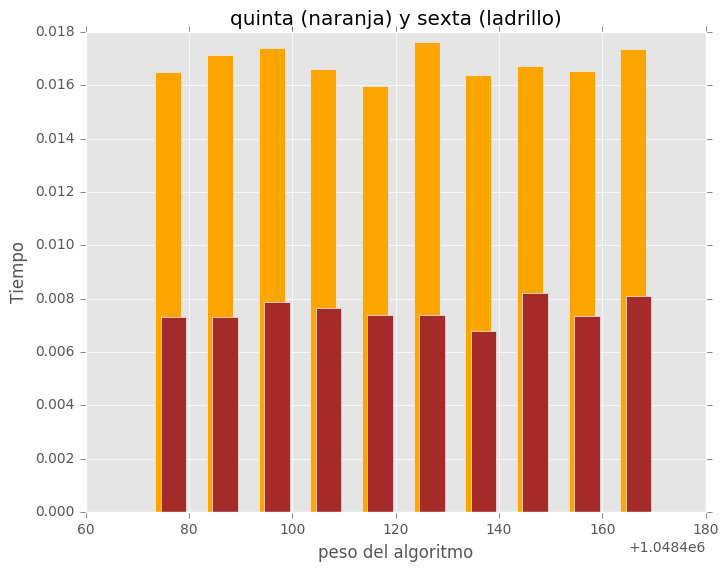
\includegraphics[scale=0.6]{5y6p.png}
	\caption{5y6	\label{5y6p}}
\end{figure} 
\begin{figure}[!hbp]
	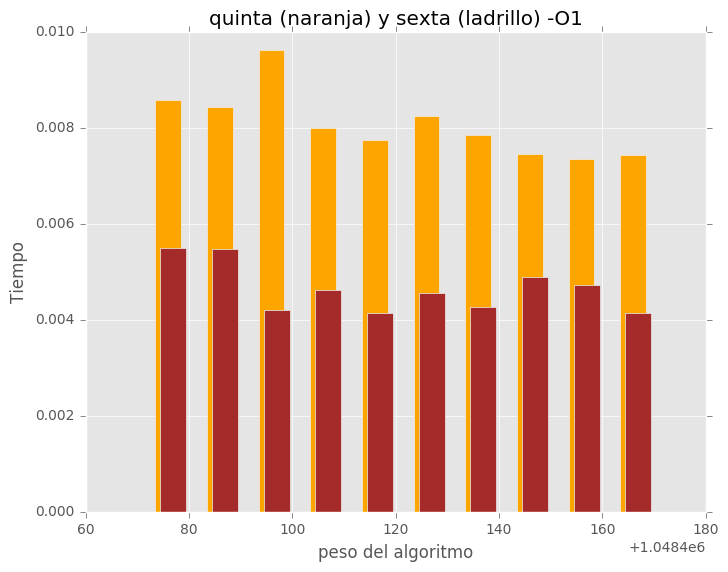
\includegraphics[scale=0.6]{5y6p_1.png}
	\caption{5y6	\label{5y6p_1}}
\end{figure} 
\begin{figure}[!hbp]
	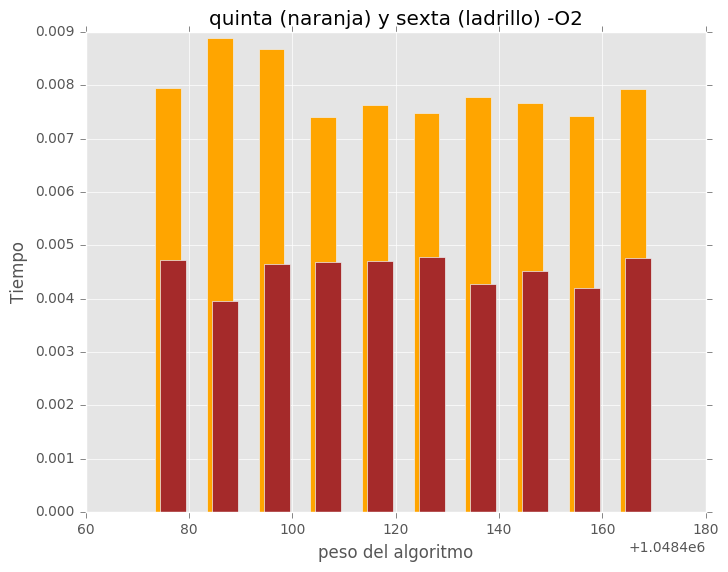
\includegraphics[scale=0.6]{5y6p_2.png}
	\caption{5y6	\label{5y6_2}}
\end{figure}
\begin{figure}[!hbp]
	\lstinputlisting[language=c]{pquinta.c}
	\caption{Código de la sexta versión (parity)	\label{parity sexta versión}}
\end{figure}

\pagebreak

\appendix
\section{Conclusiones.}
En conclusión, el aprendizaje obtenido de esta práctica bien podría ser que es muy complicado superar al compilador de C en lo que a optimización se refiere, pero es posible. He podido comprobar que, por lo general, resulta absurdo plantear un problema (por pequeño que sea) como un programa completo en ensamblador, mientras que sí que resulta práctico (sólo en ocasiones y si se tiene muy claro el objetivo y el modo de llegar a este) añadir algunas funciones en ensamblador o incluso instrucciones ASM in-line. También he podido comprobar de forma gráfica hasta qué punto puede mejorar el rendimiento de un programa en función de los niveles de optimización utilizados al compilarlo, así como ver algunos de los mecanismos que utiliza gcc para mejorar las implementaciones de nuestros algoritmos (por ejemplo, desenrollar bucles). 

\section{Script utilizado para las comparaciones}

Para realizar la práctica se me ocurrió escribir un script en Python (ya que es un lenguaje muy versátil y relativamente sencillo de entender y/o aprender) que me permitiera medir los tiempos de dos implementaciones de un mismo programa y obtener una gráfica comparándolos. El script está pensado para programas que acepten un argumento que será el peso del problema (en este caso, el tamaño del vector) y lleva a cabo 10 ejecuciones de cada programa con pesos muy similares para poder mostrar variaciones puntuales. A la hora de insertar un gráfico en el documento me he decantado por obtener dos o tres con el script y luego elegir el que más uniforme me parecía. También he intentado utilizar el script para generar los gráficos en momentos en los que mi ordenador estaba lo menos sobrecargado posible.

el script en cuestión:

\lstset{escapechar=@,style=customPY}

\begin{figure}[!hbp]
	\lstinputlisting[language=Python]{compare.py}
	\caption{Código del script para obtener las gráficas.}
\end{figure}


\end{document}